\chapter{Reti Logiche e Combinatorie} 

\section{Alcuni componenti standard}

Le tabelle di verità che vediamo si convertono in reti logiche. Una tabella di verità con $ n $ ingressi ha $ 2^n $ righe e corrisponde ad un componente logico di un circuito con $ n $ input. Vediamo alcuni oggetti utili. Ricordiamo che i passaggi per definire un componente in forma di rete logica sono: 

\begin{enumerate}
	\item Definizione della funzione con tabella di verità
	\item Conversione della funzione normalizzata in somma di prodotti
	\item Conversione a circuito con porte AND/OR/NOT
\end{enumerate}

\paragraph{Multiplexer (k commutatore)}
Un multiplexer o commutatore è un circuito, ad esempio, con due 2 ingressi, con un ingresso aggiuntivo chiamato di \textit{controllo} che permette di alternare quale sarà l'input che verrà copiato in output.

\begin{figure}
	\centering
	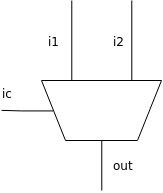
\includegraphics[]{2x1mux-gate}
	\caption{Multiplexer 2 vie 1 bit}
\end{figure}

\begin{table}[H]
	\centering
	\caption{Tabella di verità di un multiplexer a due vie da un bit}
	\label{tab:multiplexer1}
	\begin{tabular}{|lll|l|}
		\hline
		ictrl & $ in_1 $ & $ in_2 $ & out \\ \hline
		0     & 0   & 0   & 0   \\
		0     & 0   & 1   & 0   \\
		0     & 1   & 0   & 1   \\
		0     & 1   & 1   & 1   \\ \hline
		1     & 0   & 0   & 0   \\
		1     & 0   & 1   & 1   \\
		1     & 1   & 0   & 0   \\
		1     & 1   & 1   & 1   \\ \hline
	\end{tabular}
\end{table}

\begin{figure}
	\centering
	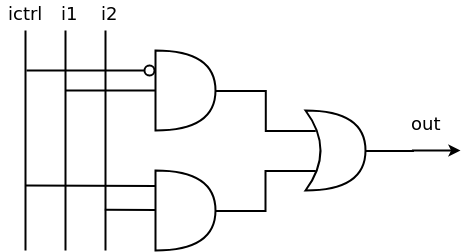
\includegraphics[width=0.68\textwidth]{2x1mux}
	\caption{Circuito logico di un Multiplexer 2 vie 1 bit}
\end{figure}



La funzione è definita come $ out = \overbar{ic} \cdot in_1 \cdot \overbar{in_2} + \overbar{ic} \cdot in_1 \cdot in_2 + ic \cdot \overbar{in_1} \cdot in_2 + ic \cdot in \cdot in_2 $ e si può ridurre in $ out = \overbar{ic} \cdot in_1 + ic \cdot in_2 $. Le tabelle di verità semplificate ci permettono di dedurre direttamente la formula ridotta. Ad esempio, la tabella seguente corrisponde a quella antecedente.
\begin{table}[H]
	\centering
	\caption{Tabella di verità semplificata di un multiplexer a due vie da un bit}
	\label{tab:multiplexer2}
	\begin{tabular}{|lll|l|}
		\hline
		ictrl & in1 & in2 & out \\ \hline
		0     & 0   & -   & 0   \\
		0     & 1   & -   & 1   \\ \hline
		1     & -   & 0   & 0   \\
		1     & -   & 1   & 1   \\ \hline
	\end{tabular}
\end{table}

\paragraph{Multiplexer a 4 Input}
Un multiplexer a 4 input ha bisogno di due bit di controllo. Avendo 6 ingressi, con porte da 8 ingressi massimo $ \implies \ceil*{ log_8(6)} $ livelli di porte.


\begin{figure}
	\centering
	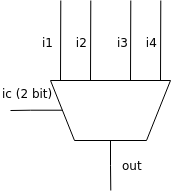
\includegraphics[]{4x1mux-gate}
	\caption{Multiplexer 4 vie 1 bit}
\end{figure}

\begin{table}[H]
	\centering
	\caption{Tabella di verità semplificata di un multiplexer a quattro vie da un bit}
	\label{tab:multiplexer3}
	\begin{tabular}{|llllll|l|}
		\hline
		$ ic_1 $ & $ ic_2 $ & $ in_1 $ & $ in_2 $ & $ in_3 $ & $ in_4 $ & out \\ \hline
		0     & 0     & 1     & -     & -     & -     & 1   \\ \hline
		0     & 1     & -     & 1     & -     & -     & 1   \\ \hline
		1     & 0     & -     & -     & 1     & -     & 1   \\ \hline
		1     & 1     & -     & -     & -     & 1     & 1   \\ \hline
	\end{tabular}
\end{table}


La formula di verità corrispondente sarà
\[ \text{out} = (\overbar{ic_1} \cdot \overbar{ic_2} \cdot in_1) + (\overbar{ic_1} \cdot ic_2 \cdot in_2) + (ic_1 \cdot \overbar{ic_2} \cdot in_3) + (ic_1\cdot ic_2 \cdot in_4)  \]

I livelli delle porte AND saranno $ log_8(n+1) $

\begin{figure}
	\centering
	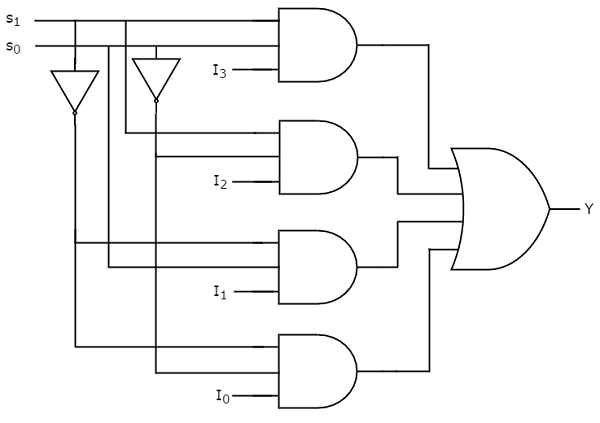
\includegraphics[width=0.75\textwidth]{4x1mux}
	\caption{Circuito logico di un Multiplexer 4 vie 1 bit}
\end{figure}

\paragraph{Commutatori (multiplexer) composti}
Un commutatore multiplo da 1 bit con un numero di vie $ y $, con $ y = 2^x \land x \in \N $ e $ y > 2 $ si può costruire a partire da un albero con $ log_2y $ livelli di multiplexer da 2 vie a 1 bit. Dove ogni bit di controllo del multiplexer complessivo controlla un livello singolo dell'albero.

\begin{figure}
	\centering
	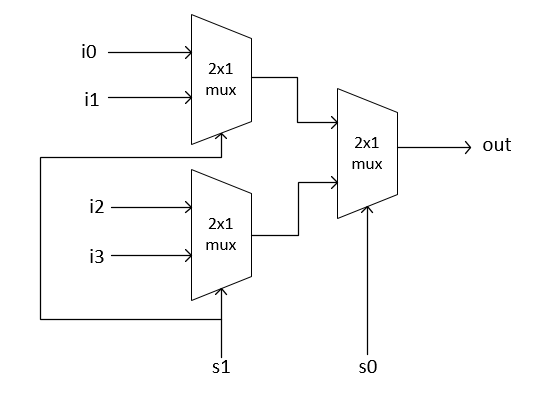
\includegraphics[width=0.75\textwidth]{4x1mux-multiple}
	\caption{Multiplexer 4 vie 1 bit composto da due Multiplexer 2x1}
\end{figure}

\paragraph{Multiplexer a 2 vie da k bit}

Un commutatore a 2 vie da $ k $ bit si costruisce con $ k $ commutatori a 2 vie ad 1 bit. Dove ogni commutatore 2x1 accetta in input le corrispettive vie di ogni bit, gli output saranno i $ k $ bit corrispondenti ad ogni Multiplexer.

% TODO multiplexer circuito da 2 vie a kbit

\paragraph{Sommatore di numeri}
Un sommatore è un componente che somma due numeri in input e restituisce in output un risultato ed un riporto.

\begin{table}[H]
	\centering
	\caption{Tabella di verità di una somma di due numeri da un bit.}
	\label{tab:sum1bit}
	\begin{tabular}{|lll|l|l|}
		\hline
		$ x_{1} $ & $ x _{2} $ & $ r_0 $ & $ z_1 $ & $r_1$ \\ \hline
		0         & 0          & 0       & 0       & 0     \\
		0         & 0          & 1       & 1       & 0     \\
		0         & 1          & 0       & 1       & 0     \\
		0         & 1          & 1       & 1       & 0     \\
		1         & 0          & 0       & 1       & 0     \\
		1         & 1          & 0       & 0       & 1     \\
		1         & 0          & 1       & 0       & 1     \\
		1         & 1          & 1       & 1       & 1     \\ \hline
	\end{tabular}
\end{table}

% TODO circuito ad 1 bit e 2 bit

Analogamente ai commutatori si possono costruire sommatori di 2 numeri a più bit a partire da sommatori di 2 numeri da 1 bit.


\paragraph{Esercizio}
Realizzare la tabella di verità e circuito di un demultiplexer a 2 vie da 1 bit. 